\documentclass{article}
\usepackage[T1]{fontenc}

\usepackage{graphicx}
\usepackage{listings}
\begin{document}

\title{FOSS Lab Report}
\author{Gokul K\\[2\baselineskip]
Roll Number: 21\\[2\baselineskip]}
\date{02 February 2020}

\maketitle

\setcounter{section}{11}
\section{Shell Programming VIII}
\subsection{Aim}
Write a shell script that accepts two file names as arguments, checks if
the permissions for these files are identical and if the permissions are
identical,output common permissions and otherwise output each file
name followed by its permissions.


\subsection{Source Code}
\begin{verbatim}
    #! /bin/bash

    # Gokul K
    # Roll No: 21
    # 25-01-2020

    # Write a shell script that accepts two file names as arguments, checks if
    # the permissions for these files are identical and if the permissions are
    # identical,output common permissions and otherwise output each file
    # name followed by its permissions.

    if [[ $# -ne 2 ]]
    then
        echo "Insufficient number of arguments"
        exit
    fi

    if [[ !(-f $1) || !(-f $2) ]]
    then
        echo "Enter valid filenames"
        exit
    fi

    perm1="`stat -c %A $1`"
    perm2="`stat -c %A $2`"

    if [[ $perm1 = $perm2 ]]
    then
        printf "Common permission: %s\n" $perm1
    else
        printf "Permissions\n %s: %s\n%s: %s\n" $1 $perm1 $2 $perm2
    fi
\end{verbatim}

\subsection{Program Description}
stat -c \%A filename outputs the file permissions of the filename. Hence
perm1 and perm2 are used to store the permissions of each file and if they
have the same permissions the condition \$perm1 = \$perm2 will be true and
the common permission will be outputted. Else the permissions of both files
will be printed

\subsection{Output}
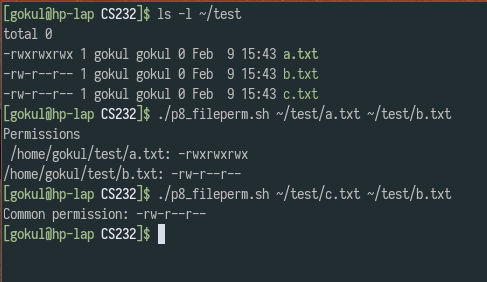
\includegraphics[width=0.9\textwidth]{img/p12.png}\newline

\subsection{Result}
The above program is run on Manjaro Linux shell. The permissions of files
are compared and consequent outputs are obtained
\end{document}